\documentclass[11pt]{article}

\usepackage[margin=2.2cm]{geometry}
\usepackage{amsmath,amssymb}
\usepackage{mathtools}
\providecommand{\llbracket}{\mathopen{[\![}}
\providecommand{\rrbracket}{\mathclose{]\!]}}
\usepackage{tikz}
\usepackage{tikz-cd}
\usetikzlibrary{arrows.meta,positioning,fit,backgrounds,calc}
\usepackage{xcolor}
\usepackage{enumitem}
\usepackage[hidelinks]{hyperref}

% ---- light colour palette ----
\definecolor{ink}{HTML}{1b2430}
\definecolor{sky}{HTML}{2f6fed}
\definecolor{leaf}{HTML}{2fa84f}
\definecolor{rose}{HTML}{d64550}
\definecolor{sun}{HTML}{e6a010}
\definecolor{mist}{HTML}{eef2f7}

\setlength{\parindent}{0pt}
\setlength{\parskip}{5pt}

\newcommand{\head}[1]{\medskip{\large\bfseries\color{ink} #1}\par\nobreak\vspace{2pt}
  {\color{sky}\rule{\linewidth}{1pt}}\par\nobreak\vspace{4pt}}

\title{\vspace{-1.4cm}\bfseries\color{ink} The Anatomy of a Verification Pearl}
\author{}
\date{}

\begin{document}
\maketitle
\vspace{-1.3cm}

\begin{center}
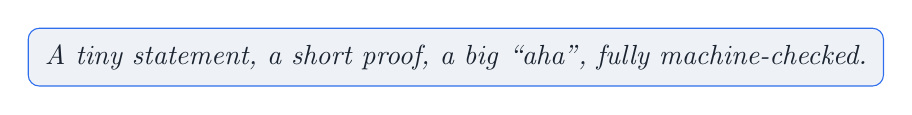
\begin{tikzpicture}[node distance=6mm]
  \node[draw=sky,fill=mist,rounded corners,inner sep=6pt] (a)
    {\color{ink}\itshape A tiny statement,\ a short proof,\ a big ``aha'',\ fully machine-checked.};
\end{tikzpicture}
\end{center}

% =====================================================================
\head{1.\ What a pearl must be}

Two boxes must both be ticked. \emph{New} on the left, \emph{beautiful} on the right.

\begin{center}
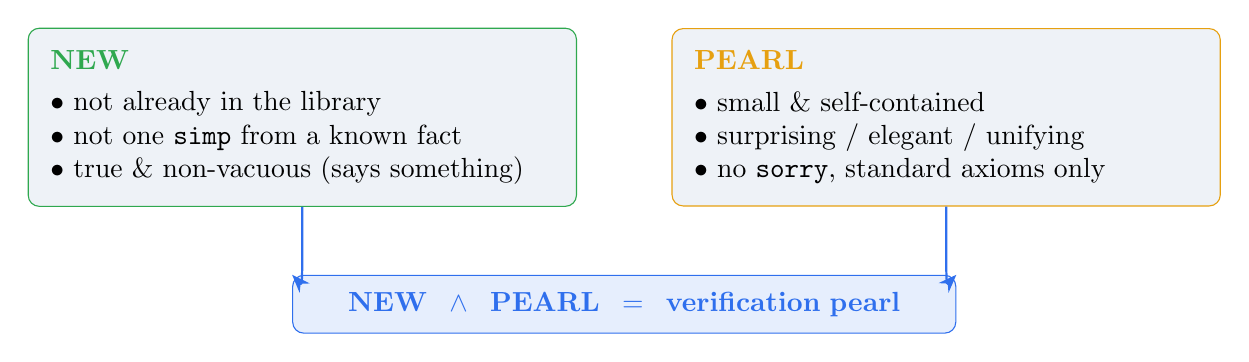
\begin{tikzpicture}[
   box/.style={draw,rounded corners,inner sep=8pt,text width=6.4cm,fill=mist},
   t/.style={font=\bfseries\color{ink}}]
  \node[box,draw=leaf] (new) {
     \textcolor{leaf}{\bfseries NEW}\\[3pt]
     $\bullet$ not already in the library\\
     $\bullet$ not one \texttt{simp} from a known fact\\
     $\bullet$ true \& non-vacuous (says something)};
  \node[box,draw=sun,right=1.2cm of new] (pearl) {
     \textcolor{sun}{\bfseries PEARL}\\[3pt]
     $\bullet$ small \& self-contained\\
     $\bullet$ surprising / elegant / unifying\\
     $\bullet$ no \texttt{sorry}, standard axioms only};
  \node[draw=sky,fill=sky!12,rounded corners,inner sep=6pt,below=20mm of $(new)!0.5!(pearl)$,text width=8cm,align=center]
     (out) {\bfseries\color{sky} NEW $\;\wedge\;$ PEARL $\;=\;$ verification pearl};
  \draw[-{Stealth[]},sky,thick] (new.south) .. controls +(0,-1.0) .. (out.north west);
  \draw[-{Stealth[]},sky,thick] (pearl.south) .. controls +(0,-1.0) .. (out.north east);
\end{tikzpicture}
\end{center}

The signature of a pearl: the ``aha'' is much bigger than the proof.

\begin{center}
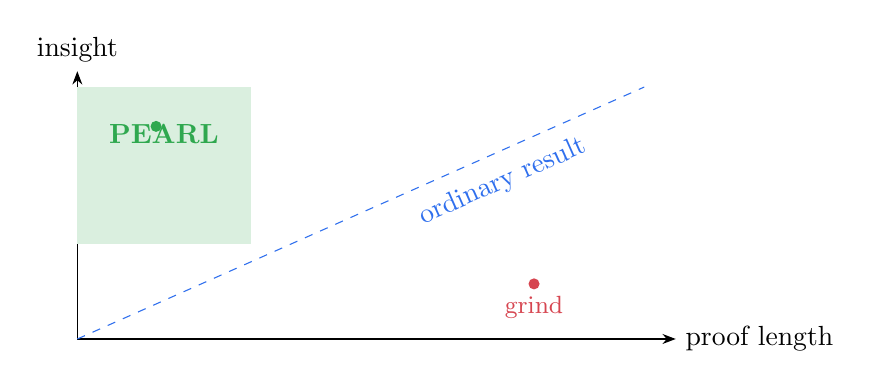
\begin{tikzpicture}
  % axes
  \draw[-{Stealth[]}] (0,0) -- (7.6,0) node[right]{proof length};
  \draw[-{Stealth[]}] (0,0) -- (0,3.4) node[above]{insight};
  % pearl region
  \fill[leaf!18] (0,1.2) rectangle (2.2,3.2);
  \node[leaf,font=\bfseries] at (1.1,2.6) {PEARL};
  % ordinary results
  \draw[dashed,sky] (0,0) -- (7.2,3.2);
  \node[sky,rotate=24] at (5.4,2.0) {ordinary result};
  \fill[rose] (5.8,0.7) circle (2pt) node[below=1pt,rose,font=\small]{grind};
  \fill[leaf] (1.0,2.7) circle (2pt);
\end{tikzpicture}
\end{center}

% =====================================================================
\head{2.\ Seven roads to a pearl}

\begin{center}
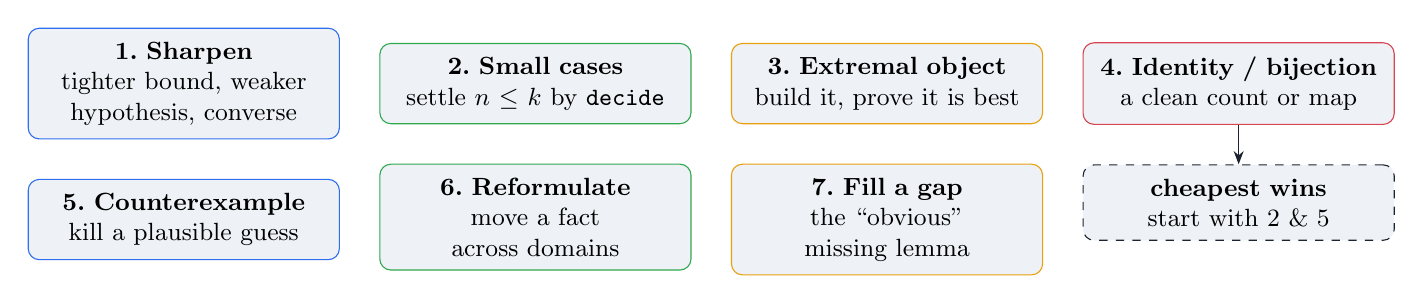
\begin{tikzpicture}[
  n/.style={draw,rounded corners,fill=mist,inner sep=5pt,text width=3.6cm,align=center,font=\small},
  every node/.style={font=\small}]
 \node[n,draw=sky]   (a) {\textbf{1.\ Sharpen}\\ tighter bound, weaker hypothesis, converse};
 \node[n,draw=leaf,right=5mm of a] (b) {\textbf{2.\ Small cases}\\ settle $n\le k$ by \texttt{decide}};
 \node[n,draw=sun,right=5mm of b] (c) {\textbf{3.\ Extremal object}\\ build it, prove it is best};
 \node[n,draw=rose,right=5mm of c] (d) {\textbf{4.\ Identity / bijection}\\ a clean count or map};
 \node[n,draw=sky,below=5mm of a] (e) {\textbf{5.\ Counterexample}\\ kill a plausible guess};
 \node[n,draw=leaf,below=5mm of b] (f) {\textbf{6.\ Reformulate}\\ move a fact across domains};
 \node[n,draw=sun,below=5mm of c] (g) {\textbf{7.\ Fill a gap}\\ the ``obvious'' missing lemma};
 \node[n,draw=ink,dashed,below=5mm of d] (h) {\textbf{cheapest wins}\\ start with 2 \& 5};
 \draw[-{Stealth[]},ink] (d) -- (h);
\end{tikzpicture}
\end{center}

% =====================================================================
\head{3.\ The worked pearl: Peirce's law has no term}

\textbf{Claim.} In the simply typed $\lambda$-calculus there is \emph{no} closed term of type
\[
  \bigl((p\to q)\to p\bigr)\to p \qquad\text{(Peirce's law).}
\]
It is a \emph{classical} tautology, yet \emph{intuitionistically} unprovable --- so no program has that type. This is road \textbf{5} (counterexample) proved by road \textbf{6} (reformulate into algebra).

\smallskip
The plan, on one line:

\begin{center}
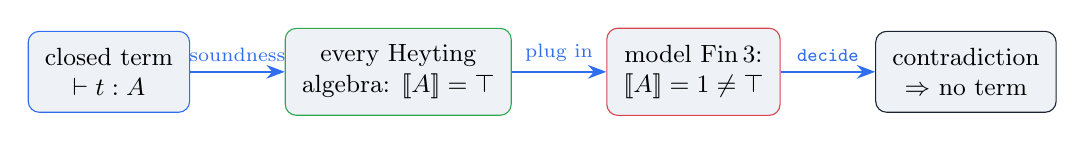
\begin{tikzpicture}[
   b/.style={draw,rounded corners,inner sep=6pt,fill=mist,font=\small,align=center},
   a/.style={-{Stealth[]},thick,sky}]
  \node[b,draw=sky]  (t) {closed term\\ $\vdash t : A$};
  \node[b,draw=leaf,right=12mm of t] (s) {every Heyting\\ algebra: $\llbracket A\rrbracket=\top$};
  \node[b,draw=rose,right=12mm of s] (m) {model $\mathrm{Fin}\,3$:\\ $\llbracket A\rrbracket = 1 \ne \top$};
  \node[b,draw=ink,right=12mm of m] (x) {contradiction\\ $\Rightarrow$ no term};
  \draw[a] (t) -- node[above,font=\scriptsize\color{ink}]{soundness} (s);
  \draw[a] (s) -- node[above,font=\scriptsize\color{ink}]{plug in} (m);
  \draw[a] (m) -- node[above,font=\scriptsize\color{ink}]{\texttt{decide}} (x);
\end{tikzpicture}
\end{center}

No normalization theory is needed: one induction plus one finite check.

% =====================================================================
\head{4.\ The engine: syntax maps into semantics}

Curry--Howard reads \emph{types as propositions} and \emph{terms as proofs}.
The interpretation $\llbracket-\rrbracket$ is a structure-preserving bridge:
an arrow type becomes Heyting implication $\Rightarrow$, a context becomes a meet $\sqcap$.

\begin{center}
\begin{tikzcd}[column sep=large,row sep=large]
\textbf{Syntax} \arrow[r,"\llbracket-\rrbracket"]
  & \textbf{Heyting algebra } H \\
A \to B \arrow[r,"\llbracket-\rrbracket"] \arrow[u,phantom]
  & \llbracket A\rrbracket \Rightarrow \llbracket B\rrbracket \\
\Gamma \arrow[r,"\llbracket-\rrbracket"] \arrow[u,phantom,"\vdash t:"]
  & \displaystyle\bigwedge_{C\in\Gamma}\llbracket C\rrbracket
    \arrow[u,"\le\;\llbracket A\rrbracket"']
\end{tikzcd}
\end{center}

Soundness is exactly the statement that the square commutes: a derivation
$\Gamma\vdash t:A$ forces $\ \llbracket\Gamma\rrbracket \le \llbracket A\rrbracket\ $ in \emph{every} $H$.
For a closed term $\Gamma=\varnothing$, so $\top\le\llbracket A\rrbracket$, i.e.\ $\llbracket A\rrbracket=\top$.

\begin{center}
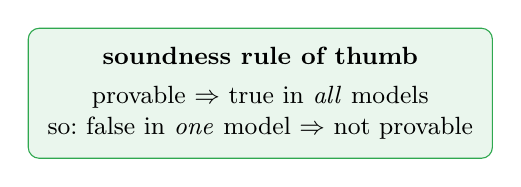
\begin{tikzpicture}[font=\small]
  \node[draw=leaf,rounded corners,fill=leaf!10,inner sep=7pt,align=center] (r) {
    \textbf{soundness rule of thumb}\\[3pt]
    provable $\Rightarrow$ true in \emph{all} models\\
    so:\ false in \emph{one} model $\Rightarrow$ not provable};
\end{tikzpicture}
\end{center}

% =====================================================================
\head{5.\ The refuting model $\mathrm{Fin}\,3$}

The smallest Heyting algebra that is not Boolean has three values
$0 < 1 < 2$ (with $2=\top$). Peirce's law evaluates \emph{below} $\top$, which
is impossible for a closed term.

\begin{center}
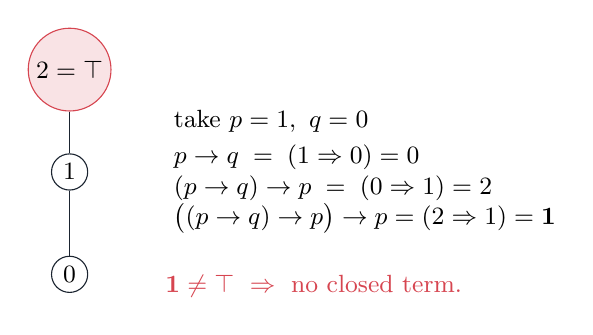
\begin{tikzpicture}[font=\small,scale=1]
  % lattice
  \node[circle,draw=ink,fill=white,inner sep=2pt] (b) at (0,0) {$0$};
  \node[circle,draw=ink,fill=white,inner sep=2pt] (m) at (0,1.3) {$1$};
  \node[circle,draw=rose,fill=rose!15,inner sep=2pt] (t) at (0,2.6) {$2=\top$};
  \draw[ink] (b)--(m)--(t);
  \node[align=left,anchor=west] at (1.2,1.3) {
    take $p=1,\ q=0$\\[2pt]
    $p\to q \;=\; (1\Rightarrow 0)=0$\\
    $(p\to q)\to p \;=\;(0\Rightarrow 1)=2$\\
    $\bigl((p\to q)\to p\bigr)\to p=(2\Rightarrow 1)=\mathbf{1}$};
  \node[rose] at (3.1,-0.15) {$\mathbf{1}\ne\top$ \;$\Rightarrow$\; no closed term.};
\end{tikzpicture}
\end{center}

Contrast: the identity $\lambda x.\,x : A\to A$ \emph{does} exist, so the type system is not empty ---
the pearl is a real distinction, not vacuous.

% =====================================================================
\head{6.\ The reusable pattern}

Every counterexample-by-model pearl has the same shape. Swap the boxes for your setting.

\begin{center}
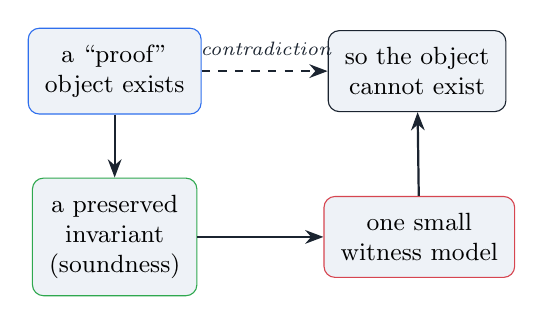
\begin{tikzpicture}[
   b/.style={draw,rounded corners,inner sep=6pt,fill=mist,align=center,font=\small},
   a/.style={-{Stealth[]},thick,ink}]
  \node[b,draw=sky]  (p) {a ``proof'' \\ object exists};
  \node[b,draw=leaf,below=8mm of p] (inv) {a preserved \\ invariant\\ (soundness)};
  \node[b,draw=rose,right=16mm of inv] (w) {one small \\ witness model};
  \node[b,draw=ink,right=16mm of p] (no) {so the object \\ cannot exist};
  \draw[a] (p) -- (inv);
  \draw[a] (inv) -- (w);
  \draw[a] (w) -- (no);
  \draw[a,dashed] (p) -- (no);
  \node[font=\scriptsize\itshape\color{ink}] at ($(p)!0.5!(no)+(0,0.28)$) {contradiction};
\end{tikzpicture}
\end{center}

\begin{center}\itshape\color{ink}
Small statement $\;\to\;$ one clean invariant $\;\to\;$ one finite witness $\;\to\;$ done.
\end{center}

\vfill
\begin{center}\footnotesize\color{ink}
Companion Lean development: \texttt{RequestProject/STLC.lean} --- builds with no \texttt{sorry}.
\end{center}

\end{document}
